\section{Machine Learning and the Medical Context}

Machine learning is the study of algorithms that can generalise solutions to problem-spaces without having been explicitly programmed them, but instead by ``learning'' from experiences, employing techniques from the fields of computational statistics, artificial intelligence, and mathematical optimisation.

One of its very first applications, Arthur Samuels coined the term ``machine learning'' to describe an automated Checkers-playing computer programme he had devised \citep{samuel_draughts}. The Samuels Checkers programme demonstrated that it was possible to have machines solve problems by implementing learning algorithms as opposed to programming solutions in ``minute detail'' in situations where doing so may be unreasonably onerous or even entirely infeasible.

Medical applications of machine learning can be found early in its history, with Earl Hunt's application of his Concept Learning System (CLS) for the purpose of medical diagnosis and prognosis as early as 1966 \citep{hunt1966}. Hunt recognised and stated that machine-learning techniques such as his CLS approach are particularly well-suited for analysing the often large amounts of data collected by medical tests, obviating time-consuming and expensive specialised investigations. The data generated by medical imaging is, in particular, both very rich and difficult to analyse in an efficient, reproducible manner. Machine learning solutions continues to be employed and further innovated for the purpose of better understanding and extracting information from medical imaging \citep{med_imaging_review}.

Machine-learning systems for medical applications are preferably of high accuracy and transparent to physicians in its methods, such that unexpected decisions are offered with an explanation that a physician can choose to agree or disagree with \citep{med_ml_review}.

The field of machine learning has given rise to a multitude of algorithms, and many of them have been applied to various clinically relevant models of detection and prognosis. Two families of machine learning that have been particularly important to the clinical context will here be surveyed, namely instance-based and perceptron-based machine-learning algorithms.

\subsection{Instance-Based Algorithms \& their Medical Applications}

Instance-based learning (IBL) algorithms are machine-learning algorithms that compare features from previous examples to unknown inputs to determine solutions. This is in contrast to other machine-learning algorithm families that generate internal generalised models of a problem-space.

%IBL algorithms typically trade classification speed and memory complexity for training speed. That is to say, training typically requires little to no processing of features and is therefore quick, but classification often requires memory and computation limited search algorithms.

Among IBL algorithms, the $k$-nearest neighbors ($k$-NN) and support vector machines (SVMs) are notable for having been widely used for a wide gamut of medical applications.

\subsubsection{The $k$-Nearest Neighbours Algorithm}

First described by \citeauthor{fix1951} while at the US Air Force as a technical report in \citeyear{fix1951}, and later formalised by \citeauthor{hart1967}, the $k$-NN algorithm is one of the early and fundamental machine learning algorithms, and is used in countless applications today.

The $k$-NN classification algorithm begins with its training step, whereby an $n_F$-dimensional feature space is created, where $n_F$ is the number of features per trained data point, all while keeping note of what class each data point in the training feature space belongs to. Subsequent classification steps involves obtaining the features for the unknown data and searching the feature-space generated in the training step for its $k$ nearest features in terms of Euclidean distance of the features, where $k$ is an odd integer. The unknown data is then classified as belonging to the same category as the majority of the $k$ nearest features.

Considered a ``lazy'' machine learning algorithm, $k$-NN requires defers heavy computation from the training stage, where no additional feature processing is required, to the classification stage, which make use of memory-complex search algorithms. Data structures such as $k\textrm{-dimensional}$ ($k$-d) trees, however, can reduce the memory and computational complexity of these searches \citep{otair2013}. This, in turn, results in a reduction of time-complexity; in the case of $k$-d trees, search is performed in $O(\log n)$ time on average.

The $k$-NN algorithm has long been used for the purpose of clinical diagnostics, with early studies being applied to microcalcification detection systems for mammography, classification of aggresivity of brain tumours, and diagnosis of pigmented skin lesions \citep{knn_microcalc,knn_braintumours,knn_skinlesions}. Clinical diagnostic tools based on $k$-NN classifiers continue to be studied, with innovation focused primarily on algorithm performance and feature engineering \citep{dhahbi2015}.

\subsection{Perceptron-Based Algorithms \& their Medical Applications}

The perceptron has a rich and storied history in the field of artificial intelligence, beginning with \citeauthor{rosenblatt1957}'s first descriptions of the algorithm in \citeyear{rosenblatt1957}. At its root, the perceptron is an algorithm to learn some linear binary classifier $f(x)$. The linear classifier trained by a perceptron takes a vector of inputs $x = \left[ x_0, x_1,\ldots,x_N \right]$ and then computes a weighted sum from a weight vector $w = \left[ w_0,w_1,\ldots,w_N\right]$ and some arbitrary bias value $b$. Sums greater than some threshold $\theta$ (typically, $\theta=0$), are classified as belonging to the first category ($f(x)=0$), or as belonging to the second ($f(x)=1$). Alternatively expressed,

$$
f(x) = \left\{
        \begin{array}{ll}
            0 & \quad \textrm{if } \left(\displaystyle\sum_{i=0}^N x_i \cdot w_i\right) + b  < \theta \\
            1 & \quad \textrm{if } \left(\displaystyle\sum_{i=0}^N x_i \cdot w_i\right) + b \geq \theta
        \end{array}
    \right.
$$

Training of the perceptron occurs by optimising the weights, which is in turn achieved by adding to the weight vector a correction value defined as the product of the difference of the desired and observed values and the input vector. A learning rate $\eta$ can be multiplied by the correction value to scale the corrections made to weights at each learning step, preventing over-corrections. For an initial weight vector $w^{t=0}$, whose elements are initialised as zero or with random values, to be trained against a training input $x_{\textrm{train}}$ with desired output $d$, we define a newly trained weight vector $w^{t=1}$ as follows:

$$w^{t=1} = w^{t=0} + \eta\left(d-f\left(x_{\textrm{train}}\right)\right)x_{\textrm{train}}$$

This weight optimisation is repeated until the weights converge. Perceptrons were met with much enthusiasm, but \citeauthor{minsky1969}'s landmark 1969 publication \textit{Perceptrons} outlined (among other limitations) the inability of perceptrons to solve problems that are not linearly-seperable, such as the exclusive-or (XOR) functions and the then infeasible computational requirements demanded by complex perceptron models. The limitations of perceptrons illustrated by \citeauthor{minsky1969} and a period of depressed AI research due to reduced funding and optimism regarding the promise of the field known as the ``AI Winter'' resulted in perceptrons being largely ignored until the later description of the backpropagation algorithm and the subsequent rise of multi-layer networks \citep{hendler2008}.

\subsubsection{Artificial Neural Networks}

Artificial Neural Networks (ANNs) are systems that overcome the linearity limitations of single-perceptron networks by connecting multiple ``hidden'' layers of perceptrons (\textit{i.e.}: multi-layer perceptron networks). The perceptrons that make up ANNs are renamed ``neurons'' in this context and their connections, ``synapses''. This new nomenclature is in reference to the biological analogy of the nervous system from which ANNs were first conceived \citep{kleene1956}.

ANNs gained in popularity when Paul Werbos described a method for accelerating ANN training through an algorithm for the backwards propagation of errors (backpropagation) from the output layer through to the connected neurons of the network \citep{werbos1982}. Hardware limitations, which \citeauthor{minsky1969} had forewarned the field about in \textit{Perceptions}, would continue to hamper their utility and adoption until advances in parallel computing, as well as in hardware in the form of graphics processing units (GPUs) would significantly speed up ANN calculations \citep{simard2005, zhongwen2005}.

ANN models have been described throughout the years to help predict breast cancer outcomes. A model described by \citeauthor{floyd1994} offered prognostic predictions given a number of features radiologists observed after mammogram such as mass size and calcification morphology (Figure \ref{fig:ann_brca}) which slightly outperformed trained physicians \citep{floyd1994}. Another ANN model had been described which out-performed TNM staging (a standard staging system which considers primary tumour size, and lymph node status) in predicting 5-year outcomes of breast cancer patients, given patient record information (age, race, payment method, etc...) as well as clinical diagnostic information (hormone status, necrosis, histological grade, etc...) \citep{burke1997}.


\begin{figure}[ht!]
	\centering
	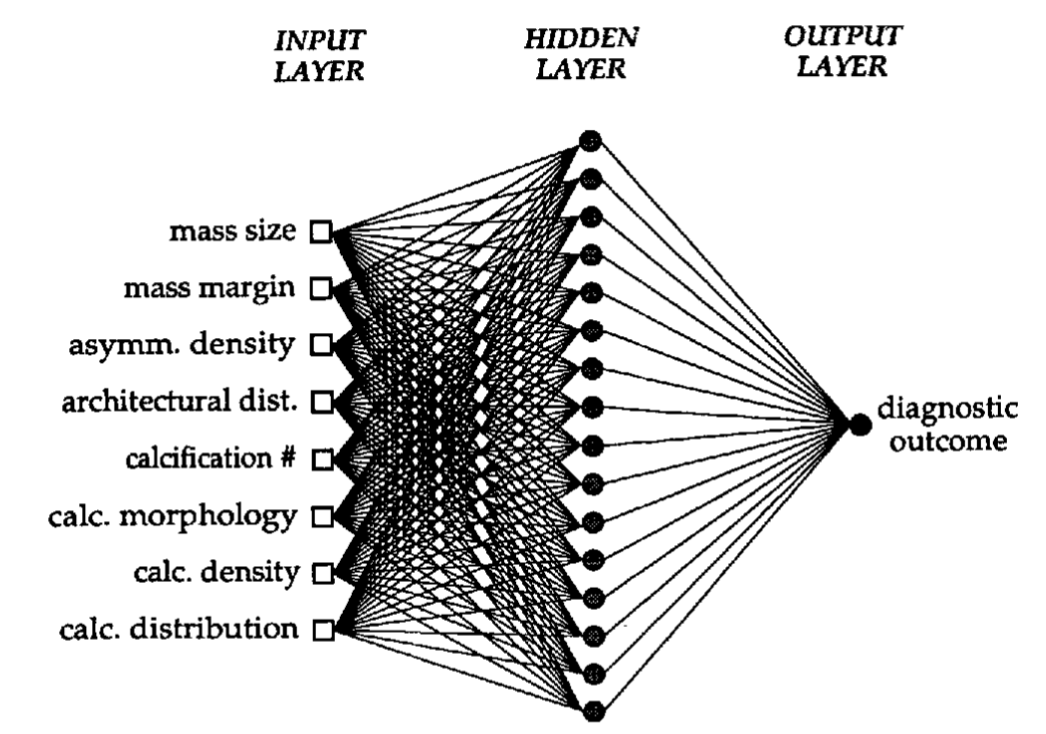
\includegraphics[width=100mm]{figures/intro/ann_brca.png}
	\caption{Architecture of the ANN described by \cite{floyd1994}. Given data interpreted by radiologists from mamograms, this multi-layer network classified benign and malignant tumours with accuracy rates that marginally outperformed trained physicians. \label{fig:ann_brca}}
\end{figure}

\subsubsection{Convolutional Neural Networks}

At the heart of an increasing amount of modern CADe/x solutions are the use of convolutional neural networks (CNNs or ConvNets) \citep{cheng2016}. ConvNets are artificial neural networks that use many hidden layers that typically either apply convolutional or pooling operations at each neuron.

This mix of convolutional and pooling layers was inspired by \citeauthor{hubel1968} who described what he called ``simple'' and ``complex'' cells in the visual cortexes of cats and monkeys. Simple cells are stimulated by patterns observed within a specific receptive field by separating the field into inhibitory and excitatory parts, comparable to the role which convolutional layers play. Complex cells, however, have no such fields and responded to stimulus on any part of the field. The behaviour of complex cells is here comparable to pooling layers, which consolidates the output of a hidden layer so that it may be passed on to a single neuron \citep{hubel1968, lecun2010}.

Models, such as most ConvNets, which make use of multiple hidden layers are described as being ``deep'', and have historically presented a significant computational challenge. An early landmark applications of ConvNets for image recognition, LeCun's character recognition model saw much success but required then-impractical computing resources to process images of resolutions much greater than $32\times32$ pixels. Recent developments in general-purpose computing on graphics processing units (GPGPU), however, have made ConvNets, whose use had previously been regarded as ``unrealistic'', practical for a wide-range of applications many years after their first conception \citep{simard2005, crick1989}. An example of being able to expand on LeCun's ConvNet architecture due to advances in hardware, VGG16 is a sixteen weight-layer ConvNet architecture (\textit{Figure \ref{fig:vgg_arch}}) that has been engineered by (and named for) the Visual Geometry Group at the University of Oxford and obtains robust accuracy rates in general image recognition tasks \citep{simonyan2014}. The VGG16 model has been shown to generalise very well to a number of different datasets, and is particularly well suited for localisation tasks, having been awarded first and second place in the classification \& localisation task of the ImageNet ILSVRC2014 contest \citep{imagenet}. This makes the use of the VGG16 architecture well-suited for the function of localisation and classification of medical imagery for the purpose of computational detection and diagnosis.

ConvNets have been successfully used to create very accurate models for the classification of breast cancer lesions. Binary models for classifying benign and malignant lesions, as well as multi-class models for distinguishing between multiple subtypes of breast lesions from H\&E stained biopsy slides have established with very high ($>90\%$) accuracy \citep{wei2017, han2017}. These models, however, are severely limited in that they classify whole imaging fields as belonging to a single class. These approaches entirely ignore the heterogeneous nature of breast lesions and are entirely ``black-boxes'' for clinicians, offering no added dimensions of information and little understanding as to why the model has interpreted a lesion the way it has. To mitigate this limitation, a classifier would be required to identify, classify and annotate sub-regions that exhibit characteristics of early lesions in medical images of breast biopsies; transparently offering insights into the classifications being made. One such method to so is to generate localisation annotations with the Gradient-weighted Class Activation Mapping algorithm. \par

\subsubsection{Localisation-Augmented Visualisation of Convolutional Neural Network Using Grad-CAM}

Recent work by \citeauthor{selvaraju2016} has made the interpretation of ConvNets much more clear by visually annotating inputs with general localisations of objects identified by the model. This technique, named Gradient-weighted Class Activation Mapping (Grad-CAM), can produce heatmaps of areas within an input image that, according to a given ConvNet model, are likely to belong to a given class. Grad-CAM is generalisable to most ConvNet architectures, and does not require to be trained on example localisation annotations.\par

Grad-CAM has been since used for the dual purpose of localising classified regions and better understanding differences between classes in practical applications ranging from plant stress phenotyping to classifying colorectal polyps \citep{ghosal2017,korbar2017}.\par

\subsubsection{Transfer-Learning for Resource Efficient Training of Neural Networks}

Two common limitations of adapting convolutional networks to domain-specific tasks such as classifying medical imagery for computer-aided detection are the large dataset and computational power requirements. These two limitations can be largely addressed by the process of transfer learning, which uses an existing convolutional architecture that has been previously trained (``pre-trained'') on a sufficiently generalised dataset appropriate for the target task \citep{transfer_learning_survey}.The ImageNet ILSVRC2014 dataset is an example of a widely-adopted, readily-available, and comprehensive general-purpose dataset that is commonly the basis of pre-trained models used for transfer-learning image classification tasks (\textit{Figure \ref{fig:imagenet_v_breakhis}a}) \citep{imagenet}.\par

Transfer learning has in-fact been used in a number of computer-aided detection, ranging from thoraco-abdominal lymph node detection and interstitial lung disease classification from chest X-ray and CT scan imaging to classification of skin cancers from dermatoscope imagery \citep{transfer_learning_lungs, transfer_learning_skin}.\par

Transfer learning uses the weights of the many hidden layers of the pre-trained network. The last fully-connected layer of the network is removed from the architecture and a new linear classifier for the network is trained on the new dataset using the pre-trained hidden layers as features.\par

A limitation of transfer learning is that the later, more specialised, hidden layers of the pre-trained network can lead to reduced accuracy of the model if the original dataset the pre-trained layer was trained against is extremely different from the new dataset. This challenge is usually met by an additional process known as fine-tuning, which continues to train the hidden layers of the pre-trained network against the new dataset using backpropagation \citep{yosinski2014}.\par

\subsection{Pattern-based Features for Classifying Medical Imaging}

Features that attempt to quantify properties of patterns have long been studied for the stated purpose of developing classifiers for medical imaging \citep{wolberg1990,meyer2004}.

Pattern detection is particularly applicable to classifying lesions from histology sections of breast tumours, where cell patterning is very significant. The observation that early lesions exhibit distinct cell patterning unique to themselves are reported in the first descriptions of hyperplasia and carcinoma \textit{in situ} of both the mammary duct and lobules by \cite{page1982}. The descriptions provided of the early lesion are strongly based on cellular architecture and patterning; distinguishing, for example, ductal and lobular carcinomas \emph{in situ} (DCIS and LCIS) from atypical ductal and lobular hyperplasias  (ADH and ALH) by ``...round, regular spacing''  in the former and their absence in the latter, sometimes exhibiting ``...swirls or streaming''.\par

\subsubsection{Gabor Filters as Texture Features}
The Gabor filter is a powerful tool for calculating texture-based features from images \citep{fan1993}. The Gabor filter comes from a family of so-called ``wavelet-transforms'', which have been shown to model the manner in which simple cells of the mammalian visual cortex are stimulated by edges in observed visual fields \citep{marcelja1980}. Gabor filters have a number of parameters, such as orientation and bandwidth, that allow them to discriminate between textures differently. Applying the Gabor filter to an image at various resolutions and with sever filter orientation parameters has been shown to produce the best results when discriminating between textures \citep{unser1995}.

